\addbibresource{reference.bib}

\chapter{Atlas TPX}\label{atlas}
Atlas TPX je síť 15\footnote{V průběhu LS3\textsuperscript{\ref{ls}} (plánováno 2017 - 2018) je plánováno rozšíření teto sítě o nové detektory} hybridních pixelových detektorů typu Timepix \ref{det:tim}, nainstalovaných na různé pozice experimentu Atlas na LHC\footnote{z angl. Large Hadron Collider} v CERN během LS2\footnote{\label{ls}z angl. long shutdown - dlouhodobá technologická přestávka LHC} (leden 2013 až březen 2015) je následníkem svého předchůdce - sítě Atlas MPX (viz \ref{atlas:mpx}). Hlavní motivací výměny této sítě bylo využití nových technologií, především pak nového detekčního čipu Timepix. Ten na rozdíl od svého předchůdce Medipix2 \ref{det:med} umožňuje rozšíření naměřené informace i o časovou oblast (viz \ref{det:tim}). To nově umožňuje provozovat detektory v módech TOA\footnote{z angl. Time of Arrival - čas příletu částice v hodinových cyklech detektoru od začátku akvizice} a TOT\footnote{z angl. Time Over Treshold - počet hodinových cyklů, kdy komparační napětí je větší, než referenční (ekvivalent energie deponované částice, viz kapitola \ref{calib})}. 

Další změnou oproti svému předchůdci je, že každý detektor obsahuje dva detekční čipy s tloušťkami $300~\mu m$ a $500~\mu m$, umístěné předními stranami k sobě - viz \ref{fig:tpx_detector_layers}. To přináší možnost měřit koincidence. Když částice projde oběma vrstvami  detektoru a zároveň v každé nechá jisté měřitelné množství své energie, je detekována oběma vrstvami a je možné zpětně zrekonstruovat její trajektorii. Tyto koincidence se nejsnáze detekují, pokud oba Timepix čipy pracují v módu TOA - jelikož rychlost částic se blíží rychlosti světla, je vysoce pravděpodobné, že zasažené pixely budou mít stejnou hodnotu.


\begin{figure}[th]
	\begin{center}
		\begin{subfigure}{6cm}
			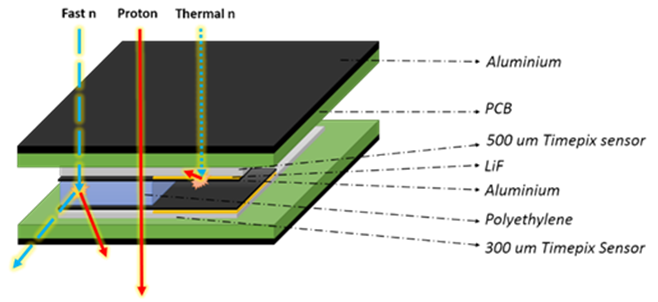
\includegraphics[width=6cm]{figures/tpx_lay.png}	
			\caption{Vrstvy detektoru}
			\label{fig:tpx_detector_layers}
		\end{subfigure}
		\hspace{0.5cm}
		\begin{subfigure}{5cm}
			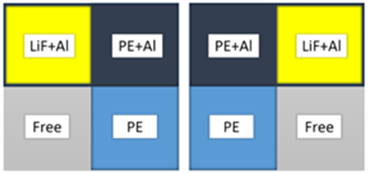
\includegraphics[width=5cm]{figures/tpx_conv.png}
			\caption{Rozmístění konvetorů}
			\label{fig:tpx_detector_convertors}
		\end{subfigure}
		\caption{Atlas TPX detektor - vrstvy a rozmístění konvertorů}
		\label{fig:tpx_detector}
	\end{center}			
\end{figure}

Mezi vrstvami detektoru je umístěn konvertující materiál pro detekci termálních a rychlých neutronů. Rozmístění těchto konvertorů je na obrázku \ref{fig:tpx_detector_convertors}.

Hlavním úkolem Atlas TPX je online monitorování spektrální charakteristiky velice různorodého radiačního prostředí Atlas experimentu, založeny na prostorovém uspořádání sítě a (vzhledem k aktuálním módu detektoru) i informaci o deponované energii zainteragovaných částic a časovou informaci. 


Detektory, instalované blízko interakčnímu bodu, jsou rovněž použity jako monitory integrované luminozity, což je veličina, která udává počet realizovaných srážek, resp. s intenzitou svazku urychlovače. Ve \cite{wagner:o_lhc} se uvádí, že je to veličina, která v případě srážení dvou proti sobě letících svazků ukazuje, jaký je součin počtů částic v jednotlivých svazcích prolétajících jednotkovou plochou v srážkové oblasti, vynásobený počtem obletů svazků za jednotku času (nejčastěji se vyjadřuje v jednotkách na centimetr čtvereční a sekundu).

%********************************************************************************
% Atlas MPX
%********************************************************************************
\section{Atlas MPX}\label{atlas:mpx}
Atlas MPX\cite{Vykydal200935}\cite{atlasmpx} je předchůdcem detektorové sítě Atlas TPX, která v současné době je plně nahrazena. Skládala se z 16 Medipix2 detektorů, které byly instalovány na různé pozice Atlas detektoru - viz obr. \ref{fig:mpx_positions}. Hlavním cílem této sítě bylo měření vlastností radiačního pole uvnitř experimentu Atlas, jeho složení, spektroskopických charakteristik a částečně také přispěla k měření neutronů. 

\begin{figure}[ht]
	\begin{center}
		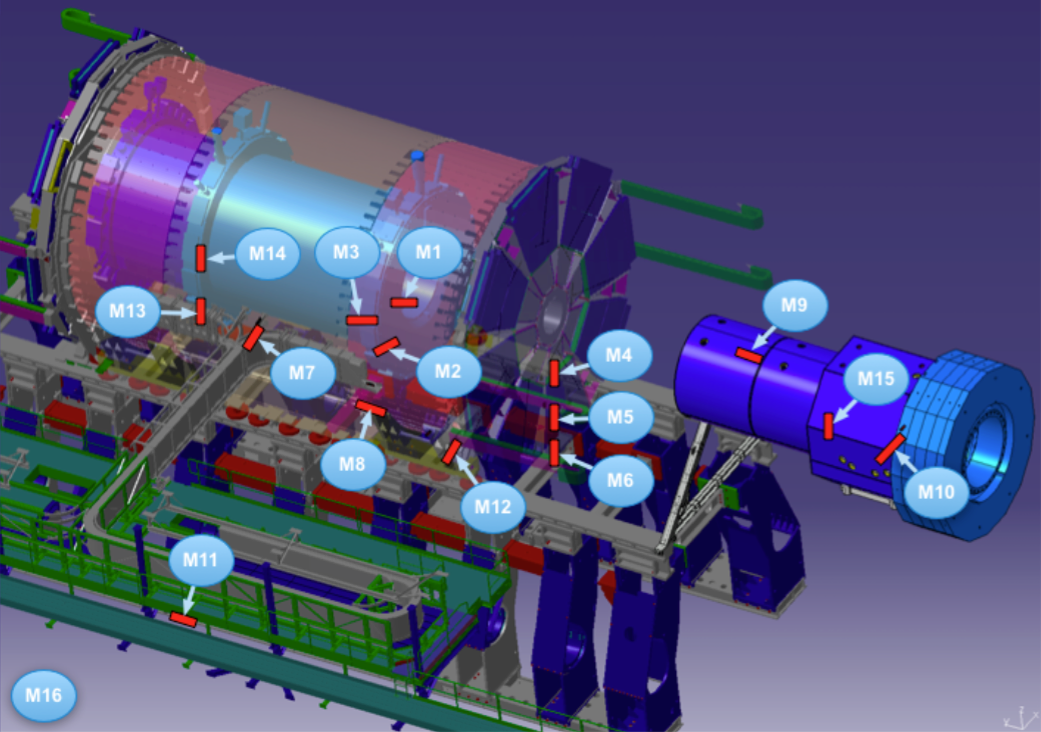
\includegraphics[width=11cm]{figures/mpx_positions.png}
		\caption{Atlas MPX s přehledem rozmístění detektorů}
		\label{fig:mpx_positions}
	\end{center}
\end{figure}

Všechny detektory operovaly v tzv. \texttt{Medipix módu}, který se vyznačují tím, že v rámci jedné akvizice počítá počet částic, které interagovaly pixelovou maticí detektoru a jejichž deponovaná energie byla vyšší, než prahová. Na obrázku \ref{fig:mpx_cluster} je znázorněn snímek z jednoho detektoru s detailem zachycených částic. Na obrázku vpravo nahoře je částice typu \texttt{heavy blob} (těžce nabitá částice, jejíž trajektorie byla kolmá s povrchem detektoru), vpravo dole je pak zachycena částice typu \texttt{heavy track} (také těžce nabitá částice, která ale přiletěla pod větším a proto zanechala větší stopu) - více klasifikaci částic se dočtete v podkapitole \ref{det:ca}.


\begin{figure}[ht]
	\begin{center}
		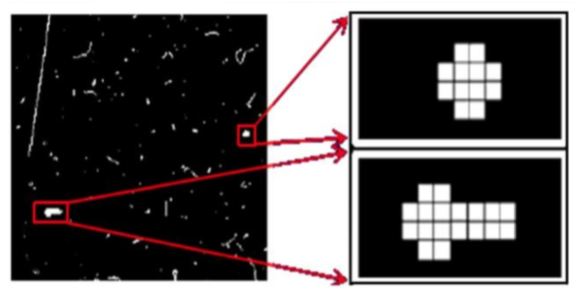
\includegraphics[width=7cm]{figures/mpx_cluster.png}
		\caption{Snímek z Atlas MPX detektoru s výřezem zachycených částic (převzato z \cite{atlasmpx})}
		\label{fig:mpx_cluster}
	\end{center}
\end{figure}


Každý z těchto detektorů byl osazen $300~\mu m$ tlustým křemíkovým senzorem, který byl pokryt konvertory pro lepší detekční účinnost neutronů (obr. \ref{fig:mpx_lay}).

\begin{figure}[ht]
	\begin{center}
		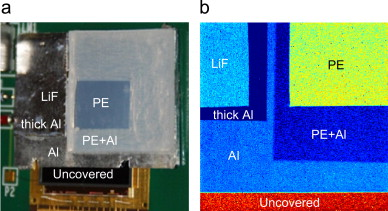
\includegraphics[width=7cm]{figures/mpx-layers.jpg}
		\caption{Fotografie znázorňující Medipix2 detektor s neutronovými konvertory (převzato z \cite{Vykydal200935})}
		\label{fig:mpx_lay}
	\end{center}
\end{figure}

\subsection{Hardwarová a softwarová architektura sítě Atlas MPX}
Tato síť se skládala z 16 \texttt{Medipix2} \ref{det:med} detektorů, které byly pomocí USB vyčítacího rozhraní \texttt{FITPix} \ref{det:fitpix} připojeny ke třem počítačům (z důvodu distribuce toku dat a výkonu). Na každém počítači se o komunikaci s detektory staral software \texttt{Pixelman} \ref{det:pixelman}, který řídil akvizici dat, nastavování parametrů detektorů apod. 

Pro vzdálené obládání každého byl vyvinut plugin pro Pixelman, který umožňoval jeho rozšíření o TCP/IP ovládací vrstvu. Pomocí jednoduchého textového protokolu bylo tedy možné řídit každý ze třech uzlů. Pro tyto účely byla vyvinuta centrální řídící aplikace \cite{Turecek2011S45}, pomocí které bylo možné řídit řídit akvizici všech detektorů a nastavovat jejich parametry. Tato aplikace poskytovala webové rozhraní (obr. \ref{fig:mpx_web}), které díky tou dobou méně striktní CERNské politiky síťové bezpečnosti bylo možné tento experiment ovládat z internetu.

\begin{figure}[ht]
	\begin{center}
		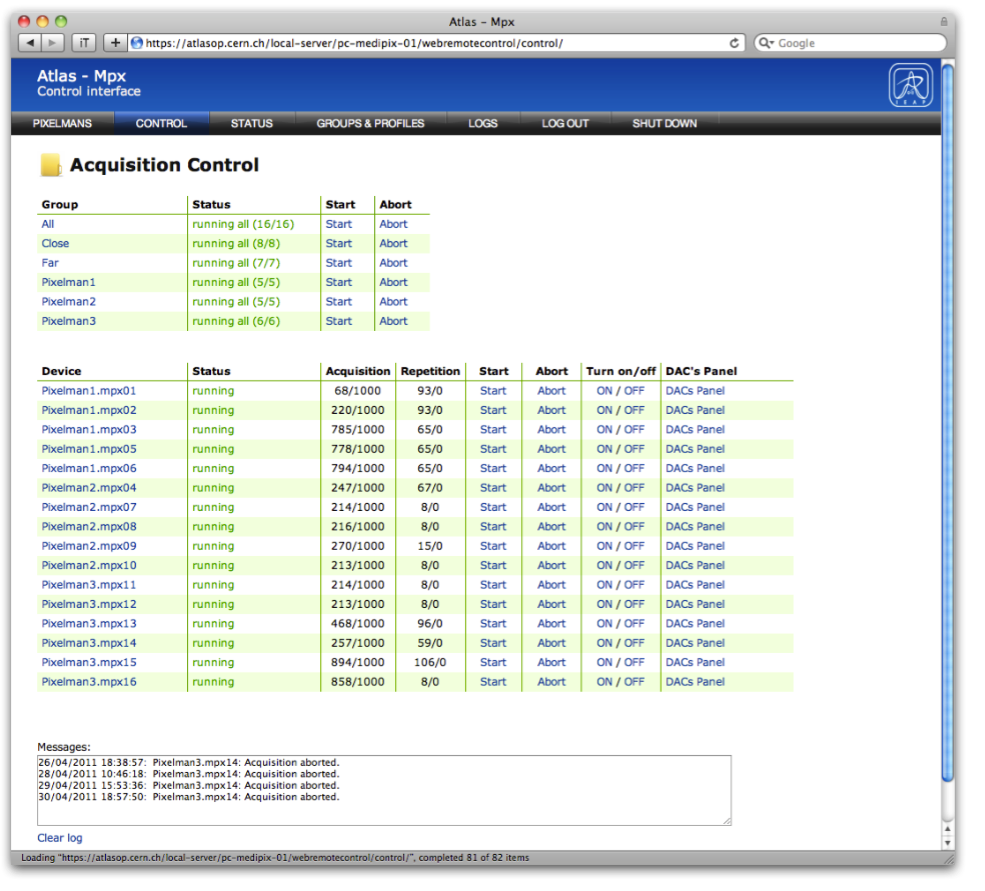
\includegraphics[width=10cm]{figures/mpx_web.png}
		\caption{Atlas MPX - řídící aplikace (převzato z \cite{TurecekThesis2011})}
		\label{fig:mpx_web}
	\end{center}
\end{figure}

%********************************************************************************
% Hardwarová architektura
%********************************************************************************
\section{Hardwarová architektura}\label{atlas:hw_arch}
Při návrhu hardwarové architekty sítě Atlas TPX musela být zohledněna zvýšená intenzita radiačního a elektromagnetického pole v okolí Atlas detektoru. Snahou proto bylo, co nejvíce hardwarových komponent umístit z dosahu tohoto pole. Z pohledu hardwarové instalace této detektorové sítě se prostory Atlas experimentu dělí na dvě části - \texttt{UX15} a \texttt{USA15} (viz obr. \ref{fig:tpx_hw_diagram}). V \texttt{UX15} se nachází vlastní experiment. V tomto prostoru byly umístěny jen vlastní detektory (na obr. \ref{fig:tpx_hw_diagram} \texttt{TPX01} až \texttt{TPX15}) a zbytek sítě je instalován v \texttt{USA15}, kterou od zbytku experimentu dělí cca $60~m$ tlustá železobetonová stěna. Tady se nachází vyčítací elektronika a další nezbytný hardware.

\begin{figure}[t]
	\begin{center}
		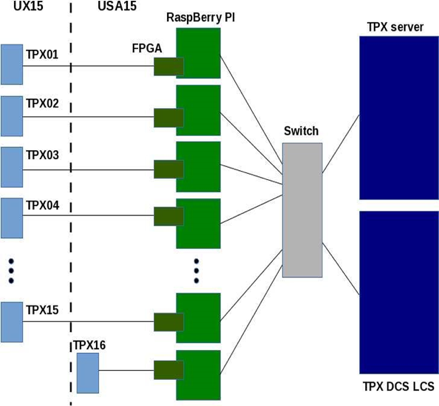
\includegraphics[width=6cm]{figures/tpx_hw_diagram.png}
		\caption{Atlas TPX - diagram hw komponent}
		\label{fig:tpx_hw_diagram}
	\end{center}
\end{figure}

Na obrázku \ref{fig:tpx_hw_foto} je fotografie  těchto komponent. Jak již bylo zmíněno výše, detektor (z obr. \ref{fig:tpx_hw_foto}, na obr. \ref{fig:tpx_hw_diagram} jako \texttt{TPX01} až \texttt{TPX15}) se skládá z dvojice detekčních čipů \texttt{Timepix2}, které jsou pomocí \texttt{LVDS} zesilovačů a cca $100~m$ dlouhých ethernetových kabelů propojeny se zařízením \texttt{AtlasPix} (obr. \ref{fig:tpx_hw_foto} dole), které vzniklo modifikací vyčítacího rozhraní \texttt{FITPix} \ref{det:fitpix}. Toto zařízení obsahuje \texttt{FPGA}\footnote{z angl. Field Programmable Gate Array (programovatelné hradlové pole)}, minipočítač \texttt{Raspberry Pi} a další podpůrnou elektroniku. 

\texttt{FPGA} se stará o komunikaci s \texttt{Timepix2} detektory, v rámci které dochází k nastavování řídících registrů \texttt{Timepix2} čipů, ovládání akvizice, vyčítání dat, řízení triggeru\footnote{řídící signál, který spouští resp. zastavuje (dle konfigurace) akvizici detektoru} apod.

\begin{figure}[t]
	\begin{center}
		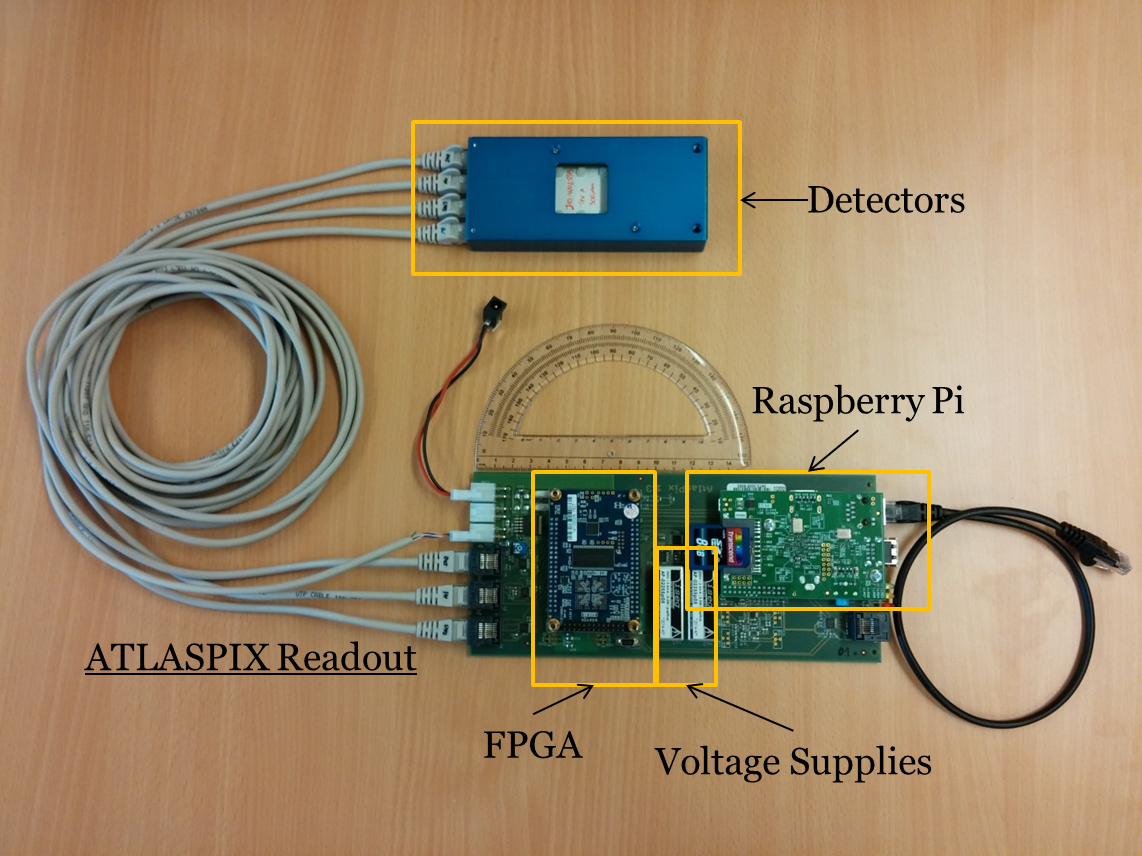
\includegraphics[width=8cm]{figures/tpx_hw_foto.png}
		\caption{Atlas TPX - fotografie hw komponent}
		\label{fig:tpx_hw_foto}
	\end{center}
\end{figure}

Dalším článkem tohoto řetězce je minipočítač \texttt{Raspberry Pi}, který plní dvě úlohy. Tou první je komunikace s \texttt{FPGA} pomocí \texttt{SPI}\footnote{z angl. Serial Peripheral Interface (sériové periferní rozhraní)} rozhraní, deserializace (získání dat ze struktury komunikačního protokolu) a derandomizace (není zaručena časová posloupnost) surových dat z \texttt{FPGA}. Druhou úlohou tohoto zařízení je poskytování API\footnote{z angl. Application Programming Interface (aplikační programovací rozhraním)} vyšším řídícím vrstvám této sítě pomocí specifikovaného komunikačního protokolu a klasického ethernetového rozhraní.

Všechny tyto zařízení jsou pomocí ethernetového switche propojeny s \texttt{TPX serverem}, který je centrálním bodem této sítě, který jí pomocí řídícího softwaru \ref{atlas:cont} a komunikačního protokolu \ref{atlas:cont:det} ovládá. Zároveň je k síti připojen i \texttt{TPX DCS\footnote{z angl. Data Control System} server}, pomocí kterého jsou různé stavové informace \texttt{Atlas TPX} sítě předávány CERNu, resp. Atlas experimentu. Tyto stavové informace jsou převážně hardwarového charakteru (na př. napětí, časování apod.), ale také jsou předávána data o počtu pořízených snímků, jejich okupanci apod.

%********************************************************************************
% Softwarová architektura
%********************************************************************************
\section{Softwarová architektura}\label{atlas:sw_arch}
Na obrázku \ref{fig:tpx_sw_diagram} je znázorněn diagram návrhu softwarové architektury sítě Atlas TPX z pohledu jejího řízení, vizualizace dat a předávání stavových informací CERNu. Diagram je členěn do dvou základních částí - ATCN\footnote{z angl. ATLAS Technical Control Network} (technická síť Atlas experimentu, která je oddělena od zbytku Atlas sítě a obsahuje systémy pro vyčítání dat a pro řízení, včetně TDAQ\footnote{z angl. Trigger and Data Aquisition (trigger a akvizice dat)} a DSC \cite{Ballestrero:atlas_network_upgrade}) a CERN služby, které poskytují perzistentní úložiště dat a web server pro jejich vizualizaci.

\begin{figure}[th]
	\begin{center}
		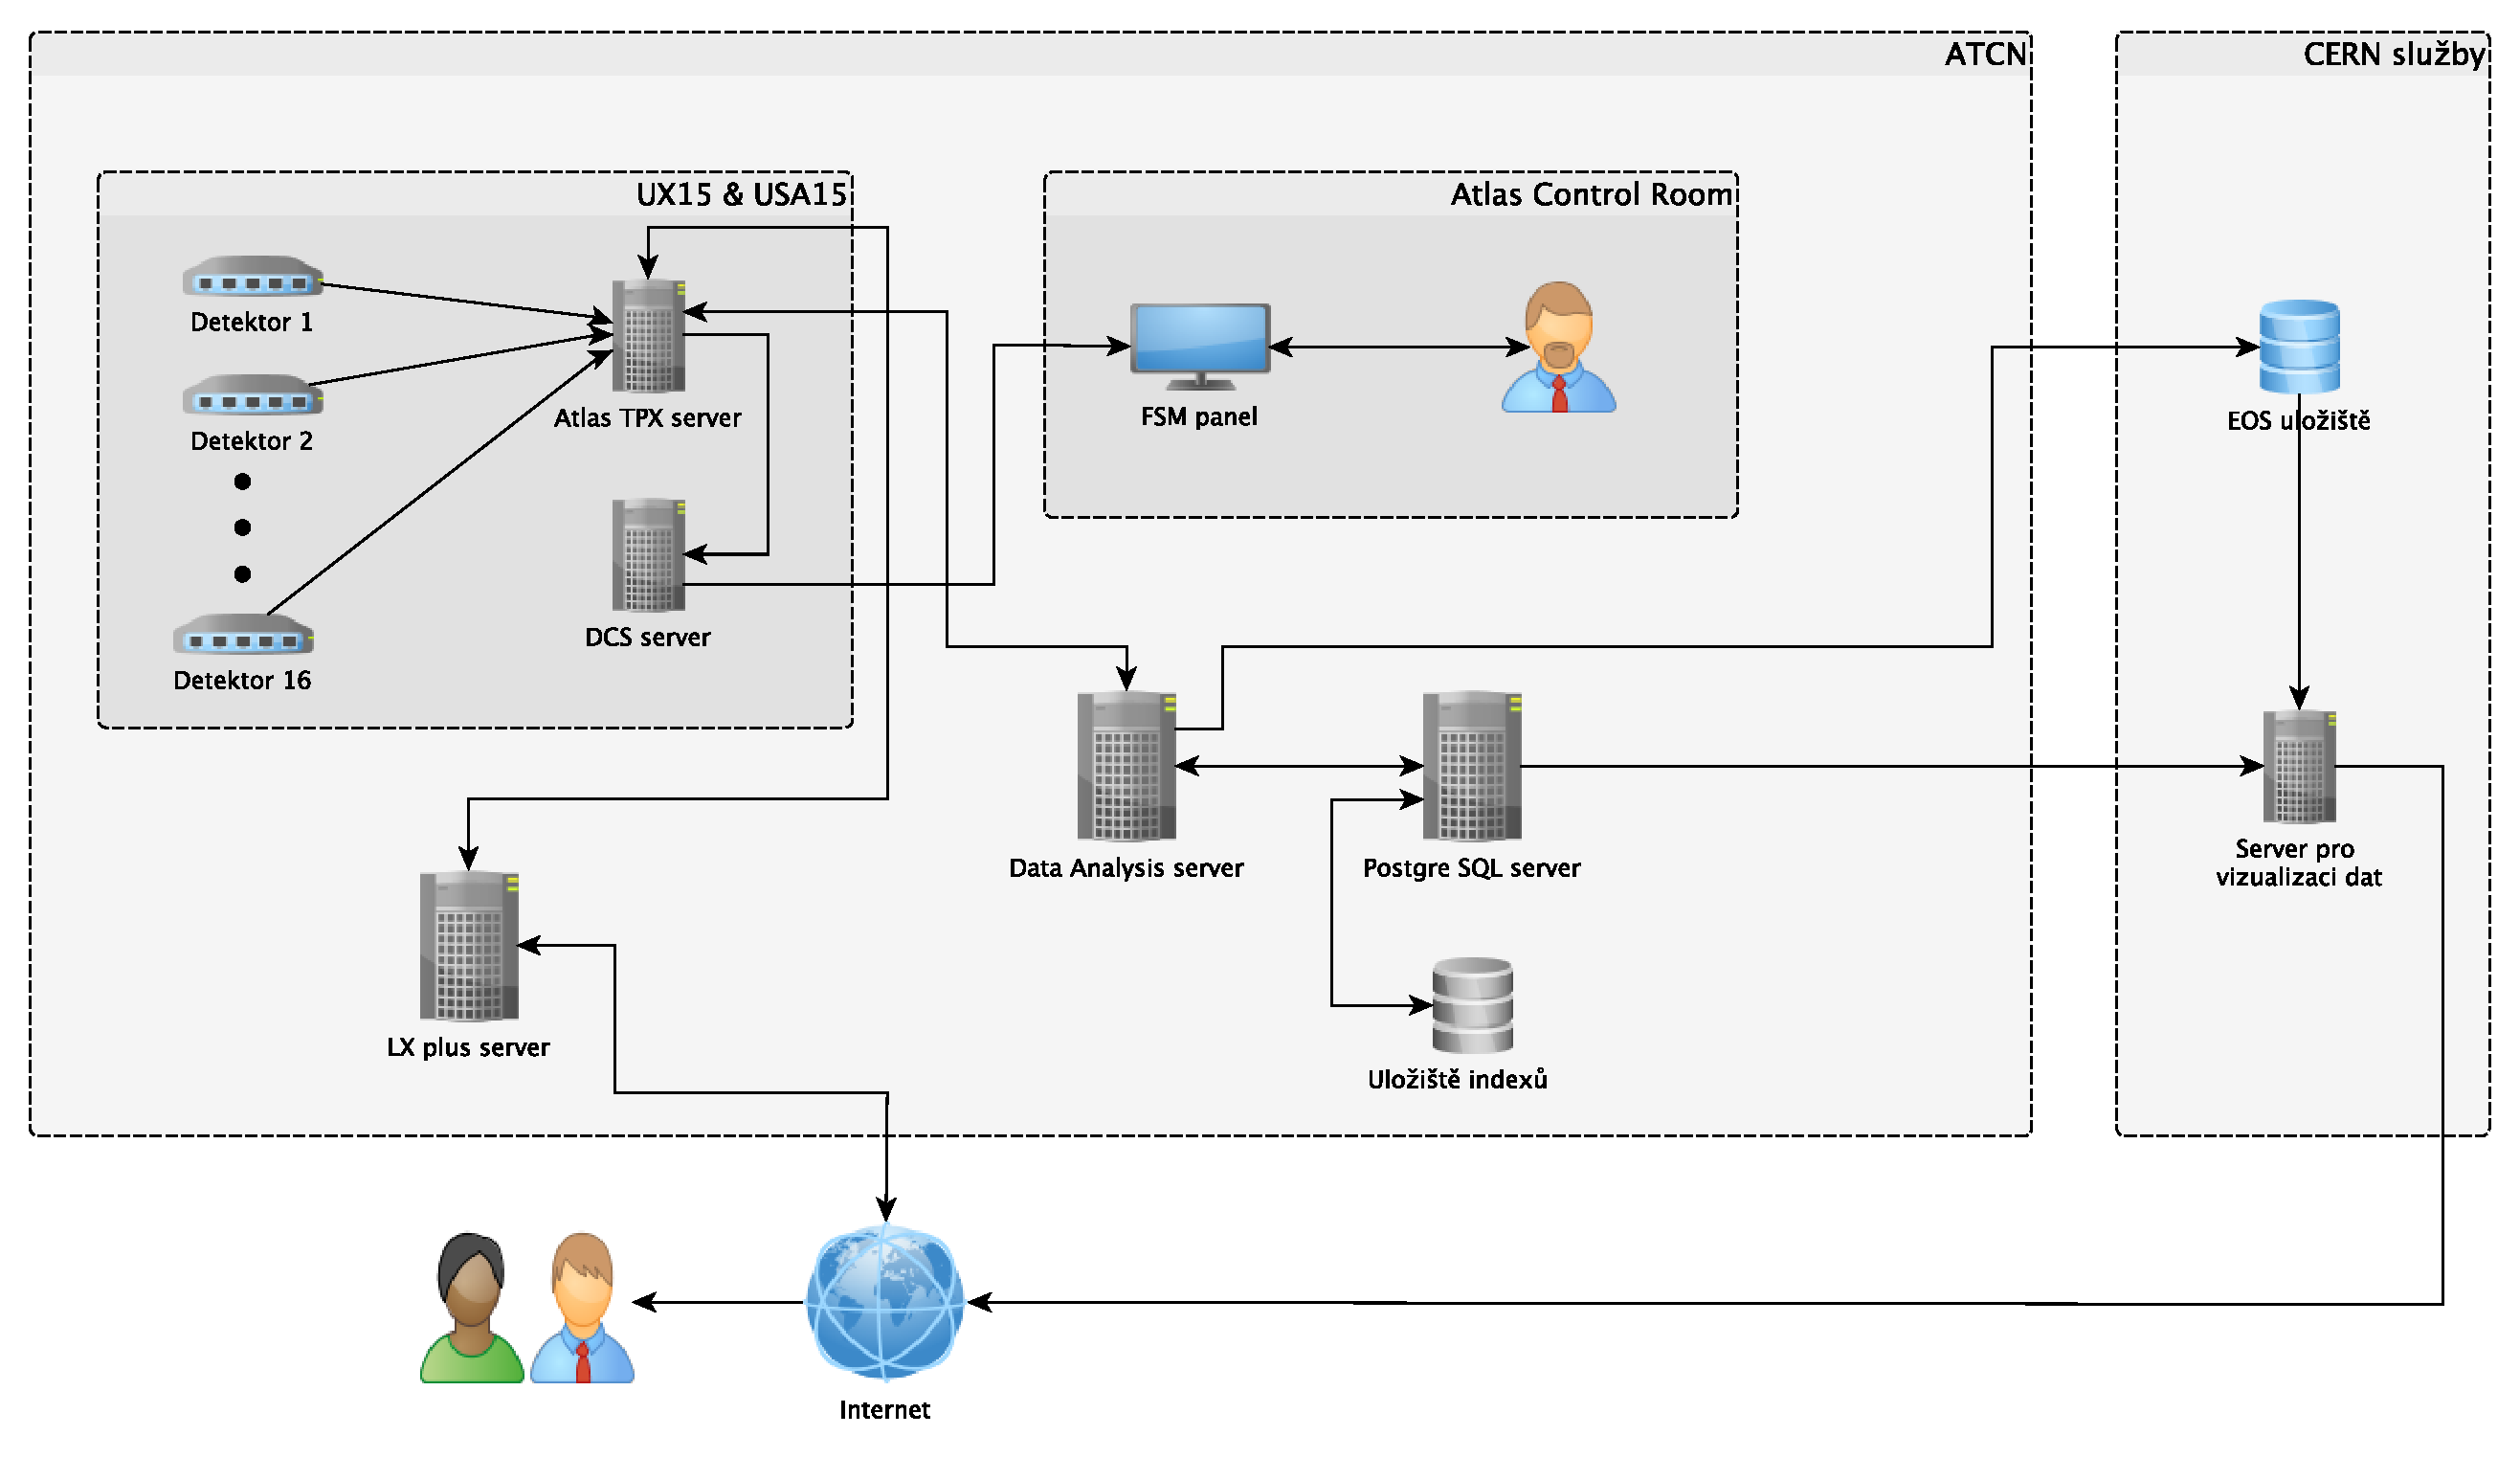
\includegraphics[width=16cm]{figures/atlas_tpx_sw_diagram.pdf}
		\caption{Atlas TPX - diagram softwarových komponent}
		\label{fig:tpx_sw_diagram}
	\end{center}
\end{figure}

\begin{description}
	\item[Popis architektury z pohledu řízení:] 
		Na obrázku \ref{fig:tpx_sw_diagram} se nachází Atlas TPX server, který je umístěn v serverové místnosti (USA15) Atlas experimentu, umístěné cca $100~m$ pod zemským povrchem. Tento server pomocí komunikačního protokolu (specifikovaném v \ref{atlas:cont:det}) řídí činnost detektorů (nastavování parametrů, ovládání akvizice apod.). Zároveň pomocí JSON REST API poskytuje rozhraní pro své řízení a předávání stavových informací (více v \ref{atlas:cont:api}). Díky tomuto rozhraní je možné činnost serveru řídit z ATCN sítě. Pro potřeby vzdáleného ovládání mimo síť ATCN slouží \texttt{LX plus server}, který zajistí spojení vytvořením SSH tunelu.\\
		Předávání stavových informací zajišťuje \texttt{DCS server}, který je od \texttt{Atlas TPX serveru} získává pomocí jeho API. Hlavním úkolem DCS je zajištění získávání stavových informací ze všech experimentů a detektorů homogenním způsobem a interakce s LHC (předávání dat luminozitě, stavu svazku urychlovače, radiační pozadí apod.). Tyto data jsou dále předávána do Atlas Control Room, která se nachází na povrchu. Tam jsou tato data operátorů prezentována pomocí \texttt{FSM} panelu, což je aplikace, která vizualizuje stromovou strukturu všech systému a detektorů Atlas experimentu. Každý list této stromové struktury (detektor, senzor atd.) má několik proměnných, z nichž každá má předem definované intervaly s příslušnými stavy (\texttt{OK}, \texttt{WARNING}, \texttt{ERROR}, \texttt{FATAL} atd.). Výhodou této struktury je, že pokud kterýkoliv list změní svůj stav, tak se tato informace propaguje přes všechny nadřazené uzly, tudíž odhalení případné chyby je pro operátory mnohem snazší.
	\item[Popis architektury z pohledu analýzy a vizualizace dat:] 
		Když kterýkoliv detektor dokončí akvizici snímku, tak vygeneruje a pošle asynchronní událost \texttt{Atlas TPX serveru} s informací, že data jsou připravena k vyčtení. Následně server vyčte snímek z detektoru (i s jeho metadaty), zpracuje a připojí k němu informace o nastavení detektoru. Poté je třeba data přenést do \texttt{Data analysis serveru}, což v principu je možné dvěma\footnote{V současné době je možný pouze první způsob, protože díky politice CERNské síťové bezpečnosti a dlouhými schvalovacími termíny je Data analysis server a všechny s ním související systémy (web server, databáze s indexem a vlastní úložiště dat) prozatím umístěn v ÚTEF ČVUT v Praze.} způsoby:
		\begin{enumerate}
			\item \texttt{Atlas TPX server} uloží získaná data v textové podobě do lokálního (či síťového) datového úložiště, odkud jsou přenesena do \texttt{Data analysis serveru} pomocí automatického kopírovacího skriptu.
			\item Druhou možností je přenesení dat pomocí JSON REST API protokolu, který je \texttt{Data analysis serverem} implementován. Tento druhý způsob je výhodnější, neb minimalizuje prodlevu mezi dobou pořízení snímku a následném zpracováním \texttt{Data analysis serverem} a dostupnosti jeho vizualizace pomocí web serveru a zároveň přináší úsporu přenesených dat.
		\end{enumerate}
		Hlavní úlohou \texttt{Data analysis serveru} provedení tzv. Cluter analýzy. Jde o proces, při kterém jsou z každého snímku získány shluky sousedních pixelů (tzv. clusterů), které mají nenulovou hodnotu. Z těchto clusterů, resp. z jejich tvaru a celkové deponované energie částice (pokud zasažení pixely operovaly v TOT módu) je možné zjistit typ částice, která danou událost způsobila. Na obrázku \ref{fig:tpx_ca} můžete vidět 6 základních dělení clusterů, kde
		 \begin{enumerate}[label=(\alph*)]
			\item je tzv. \texttt{DOT}, způsobený fotony, či elektrony o energii do $10~keV$
			\item je tzv. \texttt{SMALL BLOB}, způsobený fotony, či elektrony s energií vetšinou nad $10~keV$
			\item je tzv. \texttt{CURLY TRACK}, způsobený elektrony do $10~MeV$
			\item je tzv. \texttt{HEAVY BLOBS}, způsobený těžce nabitými částicemi (na př. alfa)
			\item je tzv. \texttt{HEAVY TRACK}, způsobený těžce nabitými částicemi (na př. protony)
			\item je tzv. \texttt{STAIGHT TRACK}, způsobený těžce nabitými částicemi (muony apod.)
		\end{enumerate}
		Po dokončení analýzy dat, jsou data uložena do \texttt{ROOT}\footnote{\url{https://root.cern.ch/}} souborů (do souborové struktury po detektorech a hodinách). Jedná se o framework, který je vyvíjený v CERN a je určený pro ukládání dat a jejich analýzu. Vygenerované soubory jsou ukládány do \texttt{EOS úložiště}, což je služba pro perzistentní ukládání \texttt{ROOT} souborů provozovaná CERN.\\
		Jelikož každý \texttt{ROOT} soubor má velikost řádově v jednotkách $GB$, jakékoliv operace nad nimi (na příklad vyhledávání) jsou velice časově náročné. Z tohoto důvodu vznikla \texttt{PostgreSQL} databáze s indexem na jednotlivé clustery, obsažené v \texttt{ROOT} souborech. 
		Pro vizualizaci dat slouží web server, který pomocí databáze s indexem a \texttt{ROOT} souborů poskytuje online výsledky cluster analýzy a další informace.
\end{description}

\begin{figure}[t]
	\begin{center}
		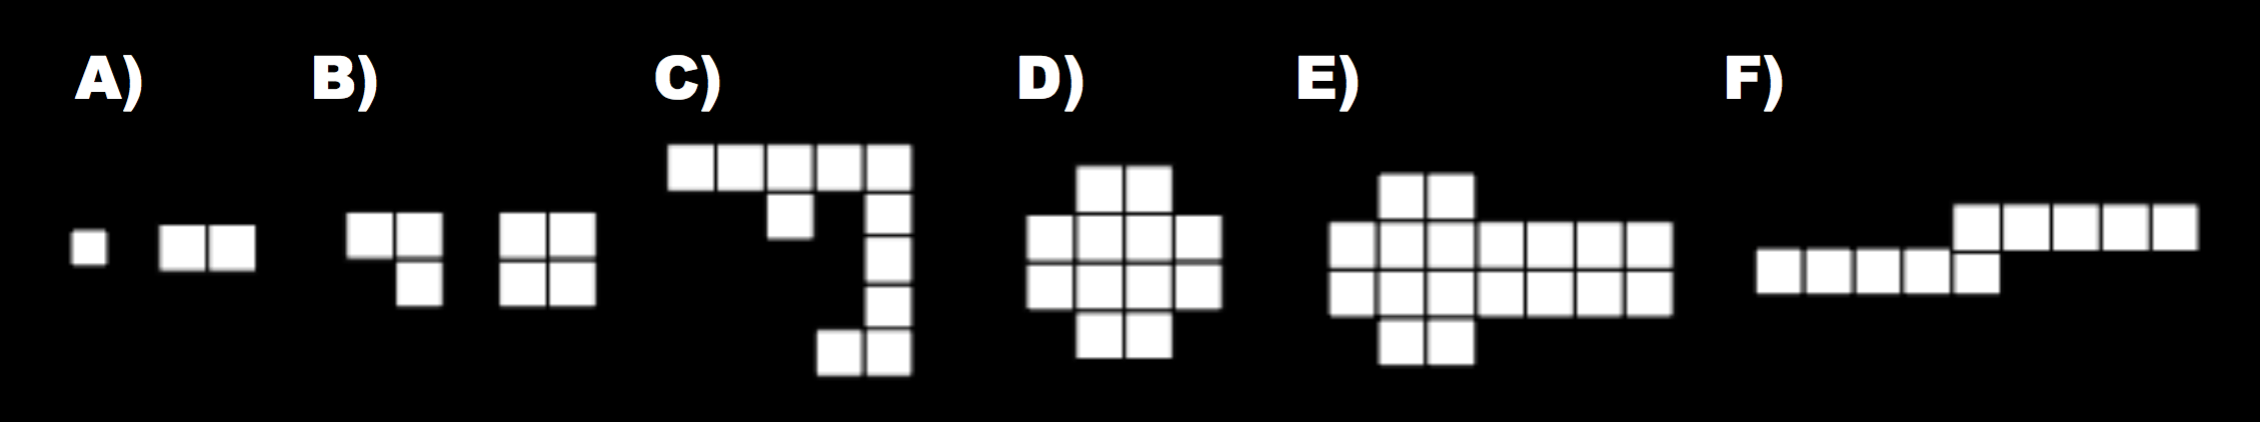
\includegraphics[width=10cm]{figures/ca.png}
		\caption{Cluster analýza - 6 základních typů clusterů (převzato z \cite{TurecekThesis2011})}
		\label{fig:tpx_ca}
	\end{center}
\end{figure}


\clearpage
\section{Řídící software}\label{atlas:cont}
\subsection{Řízení detektorů}\label{atlas:cont:det} % + komunikační protokol
\subsection{REST API server}\label{atlas:cont:api}
\subsection{Zpracování a ukládání dat}


